\documentclass[../MaxHughesThesis.tex]{subfiles}

\begin{document}
The output of the GEANT4 simulations was used to fit the beta spectrum for $b_{WM}$ and $b_{GT}$.

\section{Fitting Method}
Four GEANT4 simulations were used for the fit.
The fitting function includes the phase space, corrections, shape factor, and Fierz term and can be written as
\begin{equation}
	\frac{dN}{dE}= PS(E) \times C(E) (1 + c_{0} + c_{1} E + c_{2} E^{2} + \frac{c_{-1}}{E}) \times (1 + b_{GT}\frac{m_{e}}{E})
	\label{eq:betaspecwshape}
\end{equation}
with $PS(E)$ being the phase space, $C(E)$ the corrections, the $c_{i}$ the terms of the shape factor, and $E$ the total electron energy. 
The $PS(E)\times C(E)$ can be distributed to the shape factor, and four terms appear.
Since the $c_{i}$ and $b_{GT}$ are small, $b_{GT} \times m_{e}$ can be, to first order, added to $c_{-1}$. 
These four terms are the inputs to the GEANT4 simulaion.
These are summarized in table \ref{tab:4histfit}

\begin{table}[!hbt]
	\centering
	\caption{The four histograms used for the fits.}
		\begin{tabular}{lrr}
		Name & Formula & Normalization (when $E$ is in keV) \\ \hline
		$f(E)$ & $PS(E) \times C(E)$ & 1 \\
		$g(E)$ & $PS(E) \times E \times C(E)$ & 3.35e-4 \\
		$h(E)$ &  $PS(E)  \times E \times E \times C(E)$ & 9.89e-8 \\
		$j(E)$ &  $PS(E)/E \times C(E)$ & 2494 
		\end{tabular}
		\label{tab:4histfit}
\end{table}

Each of these pieces was generated with the same number of events.
Due to the different shapes of the spectra, a relative normalization was required.
The normalization was determined by taking the ratio of each the input spectrum of each piece compared to $f(E)$ and fitting it with the relevant power of $E$. 
These four pieces were the inputs to the GEANT4 simulation.

\section{Simulation Results Processing}
In order to use simulations results for fitting, further process had to be done in order to build the histograms for the fitting of data.
The TTrees or histograms in the output of the simulation was used.
The energy absorbed in the implant detector was filtered by the energy absorbed in the outer four gamma detectors in the simulation.
The energy gate was adjusted to match the energy gates of the data, which was the same as in the half-life measurement in table \ref{tab:GammaCuts}.
The energy gates were converted to keV using equation
\begin{equation}
        C = G \times E + b
        \label{eq:cal}
\end{equation}
where $C$ is the location of the peak in ADC channels, $G$ the gain in channels/keV, and $b$ the offset in channels.
The values of the parameters for detector calibrations are summarized in table \ref{tab:gammadetcal}.

\begin{table}[!hbt]
        \centering
        \caption{The values of the gamma calibration}
                \begin{tabular}{lrr}
                Detector & Gain (ADC Units/keV) & Offset (ADC Units) \\ \hline
                Up & 0.90 & 28 \\
                Left & 0.86 & 20 \\
                Down & 0.96 & 27 \\
                Right & 0.97 & 23
                \end{tabular}
                \label{tab:gammadetcal}
\end{table}
The two different categories of energy absorbed in the implant detector were built into two histograms.
One histogram had a condition that the energy deposited by the initial gamma ray had to be zero.
This histogram was the energy absorbed without any summing.
The second histogram was the energy absorbed where there was a contribution from the gamma ray in the implant detector.
This histogram was known as the beta-gamma sum spectrum.
These two histograms can be seen in figure \ref{fig:GEANT4Hists}.
%Maybe show some 2-D histograms here?
\begin{figure}[!htb]
        \centerline{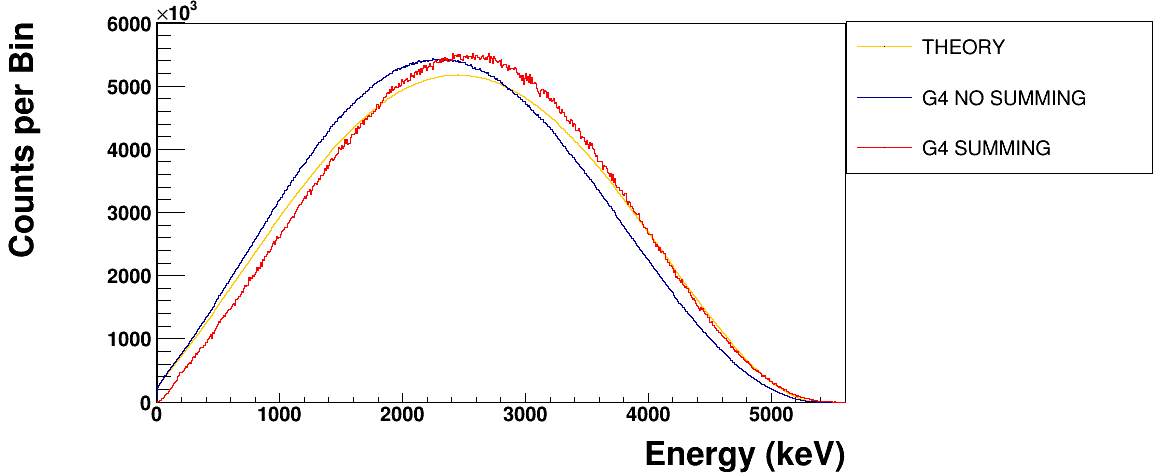
\includegraphics[width=0.78\textwidth]{GEANT4OutputBetter.png}}
        \caption{The shapes of the different histograms from the output of the GEANT4 simulation.
                 The input beta spectrum is also plotted.
                 The histograms are scaled to the same maximum.}
        \label{fig:GEANT4Hists}
\end{figure}

Another set of histograms were built with different gamma conditions.
To build the new gamma conditions, the ADC unit difference between the upper and lower gamma cuts was taken.
This was added to the old upper and lower gamma cuts to get the new gamma cuts.
The new gamma cuts were to match the data background cuts, where are shown as the red lines in figure \ref{fig:backgroundsubbeta}. 
Then, the simulation was filtered through these new cuts to build a background spectrum.
This background GEANT4 spectrum was subtracted off of the signal spectrum.
This procedure was done for all four histograms needed for the fitting procedure.
The next thing to do was to apply the detector response. 

\begin{figure}[!htb]
        \centerline{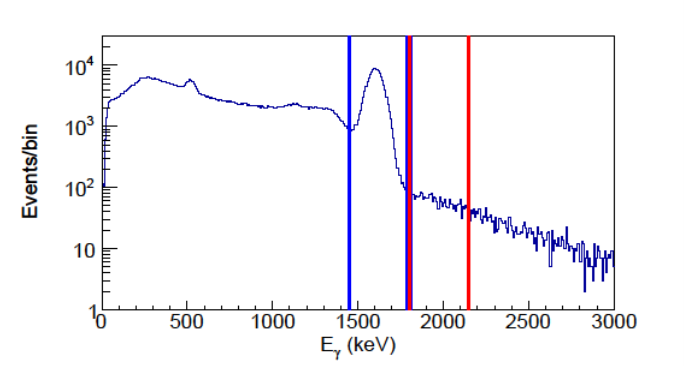
\includegraphics[width=0.78\textwidth]{BackgroundFigureUp.png}}
        \caption{A sample gamma spectrum showing the position of the gamma cuts used to build the beta spectrum.
		 The blue lines show the cuts used to build the signal spectrum.
		 The red lines show the cuts used to build the background spectrum.
                   }
        \label{fig:backgroundsubbeta}
\end{figure}
\subsection{Detector Response}
\label{sec:convolution}
Accounting for the detector resolution was done by applying a convolution function to the histograms built from the GEANT4 output files.
The convolution function was a Gaussian function. 
The $\sigma$ of that Gaussian function depended on the energy as

\begin{equation}
	\sigma(E) = A\sqrt{E}
	\label{eq:convo}
\end{equation}
where $\sigma$ was the standard deviation and $A$ a constant found through a calibration.
This was done by looping through each of the histograms' bins and reading the number of counts in each.
Then, a Gaussian distribution was built for each bin.
The center of the Gaussian was the center of each bin in keV.
The $\sigma$ of the Gaussian was calculated by using equation \ref{eq:convo}.
This Gaussian distribution was sampled as many times as there were counts in the bin.
These samples were filled into a new histogram.
This was repeated until all bins were distributed.
This was done separately for each spectrum. 

\subsubsection{Determining Detector Response}
In order to properly fit the energy spectrum, a calibration of the CsI(Na) detector had to be done.
The calibration was used to find what the detector resolution was.
Several different energy lines were used to find the calibration and the energy resolution function.
The lines were the 1.173 MeV and 1.332 MeV gammas from a $^{60}$Co source, the 0.662 MeV gamma ray from a$^{137}$Cs source, and the 0.511 MeV and 1.274 MeV gamma rays from a $^{22}$Na source.
These gamma rays were fitted with a Gaussian and a background.
The background varied from no background, a linear background, a quadratic background, and an error function background.
For the $^{60}$Co, both peaks were fit at once.
These different background gave slightly different results for the centroids and the widths of the Gaussian.
The range of the centroids and widths was taken as a systematic error.
From the centroids, the calibration for each detector was calculated with equation \ref{eq:cal}. 
This calibration curve was only used for the resolution determination.
The widths of the peaks were calibrated with the gain and plotted vs energy.
Then, equation \ref{eq:convo} was fit to the results in order to determine $A$.
The value of $A$ used for this procedure was 1.112 with an uncertainty of 0.008.

After applying the detector resolution, the pile-up in the detector had to be modeled.

\subsection{Pile-up Modeling}
In order to model the pile-up properly, a model of the detector pulses was needed. 
For the CsI(Na) signals, a linear rise and then an exponential decay was used.
The linear part went from 0 to 1 over 100 ns. 
The exponential piece started at 100 ns at 1 and decayed with a decay constant of 760 ns.
This analytic equation was scaled up or down to whatever energy was sampled.
It was then fed into a model of trapezoidal filter of PIXIE. 
The sums shown in equation \ref{eq:ensum} were done and the energy calculated.

This model was tuned on calibration data. 
A spectrum was taken of $^{137}$Cs at 25000 counts per second.
A  $^{137}$Cs spectrum taken at 2000 counts per second was used as a background and subtracted off.
Then, samples of the background-subtracted spectrum were taken up to the end of the 661 keV peak.
Monte Carlo methods were used to model the time difference between two samples.
If the two samples fell within the pile-up window, then the piled-up signal models were fed into the trapezoidal filter.
The calculated pile-up energy was saved to a histogram.
If the two samples did not fall with in the pile-up window, then they were not fed into the filter model and just filled into the histogram.
The parameters were adjusted until the generated pile-up matched the measured pile-up in the spectrum.
The results of the tuning is seen in figure \ref{fig:pileuptune}

\begin{figure}[!htb]
	\centerline{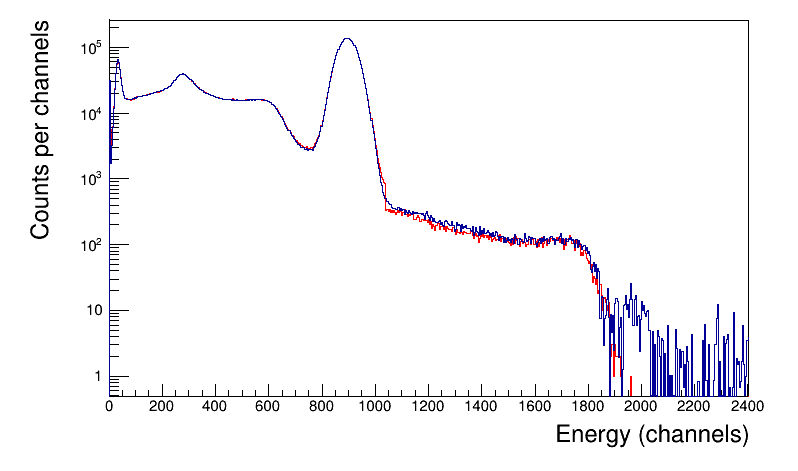
\includegraphics[width=0.78\textwidth]{PileUpTuningThesis_v2.png}}
	\caption{The tuning of the pile-up.
		 The input spectrum is in blue.
		 The generated spectrum is in red.
		 The red spectrum was generated from sampling the blue spectrum up to energy 1000 channels.
		 These samples were put through the pile-up model.}
	\label{fig:pileuptune}
\end{figure}
For the pile-up model, the resulting times are shown in table \ref{tab:tunepileupmodel}.
In addition, the parameters of the actual energy for the CsI(Na) implant detector are shown.

\begin{table}[!hbt]
	\centering
	\caption{Pile-up model parameters compared to the energy filter parameters}
		\begin{tabular}{lrr}
		Parameter & Pile-up model value & Energy filter value \\ \hline
		$\tau$ & 880 ns & 900 ns \\
		$tPEAKING$ & 880 ns & 480 ns \\
		$tGAP$ & 72 ns & 48 ns  
		\end{tabular}
		\label{tab:tunepileupmodel}
\end{table}
The $\tau$ value in the pile-up tuning is very similar to that of the energy filter.
The other parameters are roughly double in the pile-up model compared to that in the PIXIE energy filter.

The pile-up model was applied to the simulation after the detector response was applied. 
Of the four different simulations needed for a fit, only $f^{*}(E)$, $f(E)$ after applying the detector response, was fed into the pile-up model.
The amount of pile-up is small. 
Applying the pile-up to the other terms of the shape factor gives a negligible contribution.
The beta only spectrum and the beta-gamma sum spectrum of this simulation was added together and fed through the pile-up model.
With the pile-up spectrum described, all the pieces of the fit function are in place.

\subsection{Fit Function}
For the fit function, the convoluted histograms and pile-up were rebinned to a bin width of 64 keV.
Then, each of the histograms were turned into a spline. 
The five splines were fed into a fit function.
The fit function was

\begin{equation}
	H(E) = A \times [( 1 + c_{0}) f^{*}(E) + c_{1}g^{*}(E) + c_{2} h^{*}(E) + (c_{-1} + b_{GT} m_{e}) j^{*}(E)] + B \times pu^{*}(E)
	\label{eq:betafit}
\end{equation}
where $A$ is the normalization, $B$ the level of pile-up, $pu^{*}(E)$ is the generated pile-up spectrum, and $f^{*}(E),g^{*}(E),h^{*}(E),$ and $j^{*}(E)$ the different simulation results as shown in table \ref{tab:4histfit} after the convolution was applied.
In order to change the units of the x-axis in the data to energy in keV, a calibration was needed.
For this calibration, the offset was fixed in the fit function.
However, the gain of the calibration was left as a free parameter.
This was to account for gain shifts, such as an apparent rate-dependent gain shift due to the afterglow in the crystal.

In the fit, each of the $c$s were written out in terms of the nuclear form factors.
In these form factors, $b_{WM}$ was left as a potential free parameter. 
If $b_{WM}$ was fit with the fit function, $b_{GT}$ was fixed to be 0. 
If $b_{GT}$ was fit, then $b_{WM}$ was fixed to be 43.4. 
In total, the fit function had four free parameters:
$A$, $B$, the gain $G$, and either $b_{WM}$ or $b_{GT}$. 
In order to benchmark this fitting method, pseudo-data was generated and fitted.

\subsubsection{Fit Function Characterization}
Different methods of the fit function were tested. 
The first is the so-called ``hybrid method'', where only one simulation is needed.
The GEANT4 with only the phase space and corrections is generated. 
Then, it is multiplied by the shape factor.
This function was 

\begin{equation}
	H^{*}(E) = A \times f^{*}(E) \times S(E) + B \times pu^{*}(E)
	\label{eq:hybridmodel}
\end{equation}
with $A$ being a normalization constant and $S(E)$ the shape factor. 
This method of fitting is not correct, as the $E$ in $f(E)$ is not the same as the initial energy in the analytical shape factor $S(E)$. 

The first test was done just with a linear term in the psuedo-data.
An older version of the GEANT4 code had a phase space times corrections times a linear shape factor fed into it.
This psuedo-data was fit with the hybrid model.
Initially, the shape factor was applied to total energy inside the implant detector.
This was found to induce a shift of the measured linear term.
Applying the shape factor only to the beta only part of the spectrum solved this issue. 

To further test the fitting method, two more spectra were generated.
One had the nuclear shape factor with $b_{WM} = 43.4$, which was the new pseudo-data spectrum.  
The other had no shape factor.
After applying the coincidence condition to both of these simulations, the function with no shape factor was used to fit the function with the shape factor. 
The gain in these fits was left as a free parameter, and the offset was fixed to a value of 0. 
To manually check the statistical uncertainty, the pseudo-data spectrum was fluctuated.
Each bin had its content and error read. 
That bin error and content was used to build a Gaussian random number distribution.
This random number distribution was sampled, and a new bin center created.
After doing this to the entire spectrum, the new spectrum was fit.
The resulting $b_{WM}$ was recorded.
Then, $b_{WM}$ was set to 43.4, and the Fierz term fit. 
These fitted terms were saved to a histogram.
This was done 1000 times to get a spread of values.
From this, it was discovered that spline interpolation was the best way to fit the spectra.

The same method was used to see if the fitting method induced a lower beta cut effect or not. 
1000 spectra were generated by scrambling one spectrum over and over.
These spectra were fit from a lower beta cut up to the end point minus 100 keV.
The lower beta cut was varied from 200 keV up to 2 MeV.
From this it was found that this fitting method induced an effect above 1200 keV.
This effect was very large in the measurement of $b_{GT}$.

Doing the same thing with the four-histogram fitting method shown above showed that there is not such a large lower beta cut effect.
The four histogram fit is the one described above. 
More pseudo-data was generated, along with four histograms to be used for fitting.
This was largely done to get a handle of the normalization of the histograms.
The normalization was obtained by taking the ratios of the histograms and fitting them with the functional forms. 
After the normalization, the fit was done.
The output $b_{GT}$ and $b_{WM}$ obtained of the pseudo-data was the one put in.

\section{Experimental Data Processing}
After the fit function was tested and verified, the data was ready to be fit. 
For the fit, the experimental data had to be processed as well. 
The energy spectrum of the implant detector was put in coincidence with the 4 gamma detectors.
The energy cuts of the gamma detectors were the same as in the life-time measurement, as seen in table \ref{tab:GammaCuts}.
An additional condition was that only one of the gamma detectors could have fired for each event, much like the processing for the GEANT4 events.

An additional condition in the data was a time difference condition.
For this measurement, the time difference between a beta event and a gamma event had to be between -300 and 24 ns.
This captures the entire spectrum, as the time stamps are largely dependent on energy. 
Then, a 2-D histogram was built, with energy on one axis and time since last beam on on there other.
The decay cycles were 22 seconds long for the CsI(Na) implant data. 
The decay cycles were split up into 3 segments with equal number of counts.
To do this, it was assumed that the rate depended on the time as an exponential with a half-life of 11 seconds.
The time interval was split in such a way that the integral of the exponential was equal over 3 different segments.
The total time interval was from 1.5 to 22 seconds.
These splits worked out to be at 5.89 s and at 11.98 seconds. 
This 2-D histogram was projected onto the time axis between the splits in order to build the energy spectrum of the fit. 

\subsection{Background Subtraction}

A background subtraction of the data was required.
To build the background, cuts placed above the regular gamma cuts in table \ref{tab:GammaCuts} were used.
Much like in the process of the simulation spectra, the difference between the upper and lower gamma cuts were taken.
These differences were added to the original upper and lower gamma cuts to get new gamma cuts.
A beta spectrum was with a time difference condition and these new gamma cuts.
This was the background spectrum.
It was then subtracted off of the signal spectrum. 
The position of the gamma cuts on a sample spectrum is shown in figure \ref{fig:backgroundsubbeta}.


\section{Beta Spectrum Fit Procedure}
After the data was processed, the fit was done run by run.
First a prefit for each section was done to calibrate the energy from 500 channels to 6000 channels.
This was done to obtain a calibration of the data.
Then, two endpoints fixed in keV were used for the actual fit.
The fitting function with a fixed offset was fit using a maximum likelihood method.
The resulting $b_{WM}$ was recorded.
For the Fierz term fit, the $b_{WM} = 43.4$ was applied to the shape factor and the $b_{GT}$ was recorded.

The offset used for the fit was varied.
The effect of the offset will be discussed in the next section. 
The calibrated start and end of the fits were 250 keV to 7500 keV. 
A sample fit is shown in figure \ref{fig:samplefit}, where the offset was fixed to 0.

\begin{figure}[!htb]
	\centerline{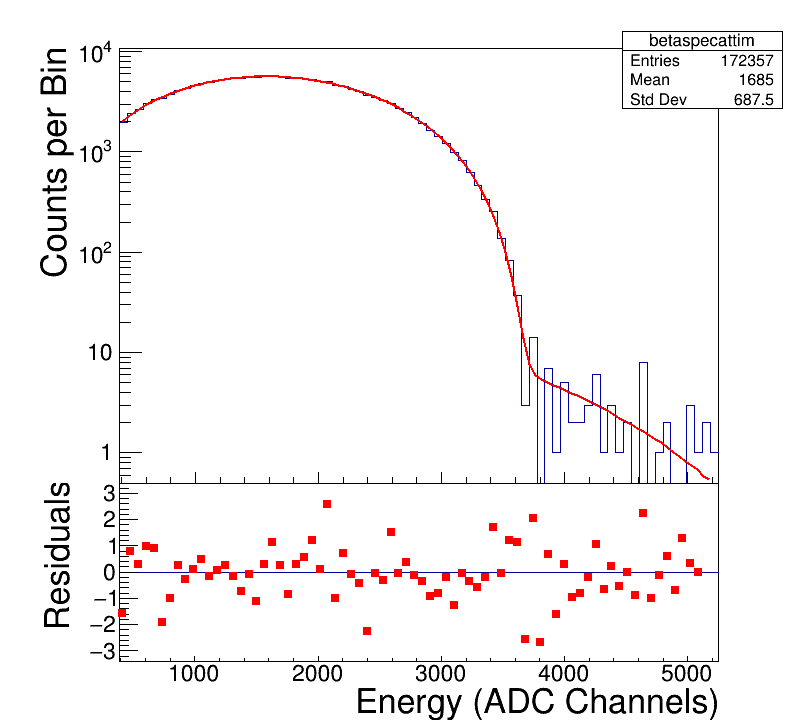
\includegraphics[width=0.70\textwidth]{CsIRun317FierzTermResids.png}}
	\caption{A sample fit of the beta spectrum. 
		 The residuals of the fit are shown below the graph}
	\label{fig:samplefit}
\end{figure}

\section{Systematic Uncertainties}

After testing the fit and fitting the data, the systematic effects were investigated.
The systematic uncertainties can be divided into three categories.
The first set are the uncertainties that have to do with the inputs to the simulation.
The second set has to do with the inputs to the fit.
The final set has to do with the uncertainties of the nuclear form factors in the shape factor. 
One of the largest systematic uncertainty has to do with the position where the fit is started. 

\subsection{Lower Beta Cut Effect}

The lower beta cut effect is the systematic shift of the fitted gain $G$ as a function of where the fit started.
The $b_{WM}$ and $b_{GT}$ are correlated with $G$ and shift as well.
There are several different input factors that can induce such an effect.

\subsubsection{The Offset}
Initially, the offset used was the offset from the calibration in equation \ref{eq:cal}.
The offset used was 10.05 ADC units.
This calibration was determined using photons instead of electrons.
%Electrons generate 2\% less light than photons \cite{REFHERE} % maybe knoll?
It also doesn't probe the same location as where the beta electrons are.

When applying an offset of 10.05 in a fit of the data, it was found that the output varied greatly as a function of where the fit was started.
For these graphs, the end of the fit (or upper beta cut) was set to 7500 keV.
The detector is known to be non-linear below 200 keV \cite{Kno10}, so any fit starting below that point is suspect. 
After 2000 keV, the shape of the beta spectrum makes getting a good fit unlikely.
The lower beta cut was varied between these two end points.
The effect in the average gains is shown in figure \ref{fig:offset10LBCeffect}.

\begin{figure}
    \centering
    \begin{minipage}{0.50\textwidth}
        \centerline{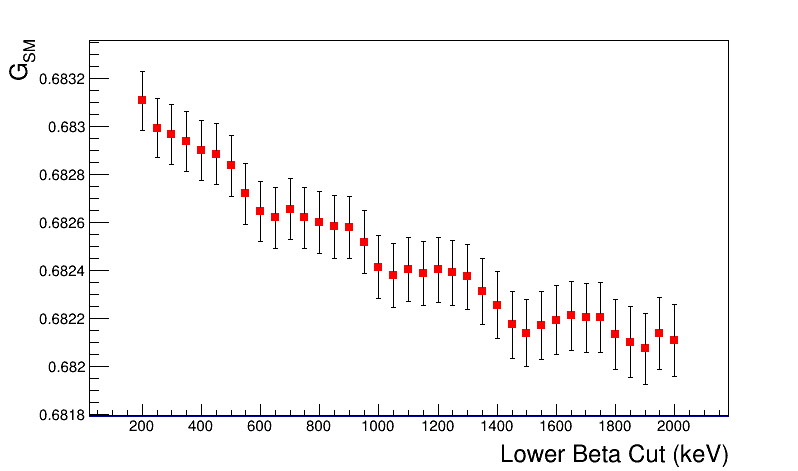
\includegraphics[width=0.9\textwidth]{CsILBCvGainSMOffsetis10p054histfit.png}}
    \end{minipage}\hfill
    \begin{minipage}{0.50\textwidth}
        \centerline{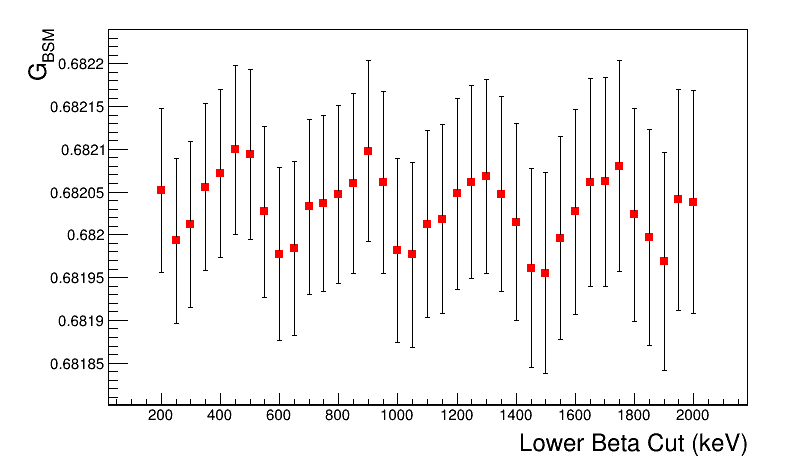
\includegraphics[width=0.9\textwidth]{CsILBCvGainBSMOffsetis10p054histfit.png}}
    \end{minipage}
    \caption{For the standard model fit, there is a large dependence of the gain on the start of the fit.
	     The offset here is 10.05.}
    \label{fig:offset10LBCeffect}
\end{figure}

To test the effect of the offset, a Monte Carlo was written.
A sample histogram with only the phase space and the shape factor was generated. 
These histograms were generated with an offset of 10 ADC units.
A random gain was applied to the psuedo-data histogram. 
Then, the fit function had a different offset applied to it.
For example, fitting the histogram generated with an offset of 10, and fit with an offset of 20 gives an effect as seen in \ref{fig:MCoffset10applied20}.

\begin{figure}
	\centerline{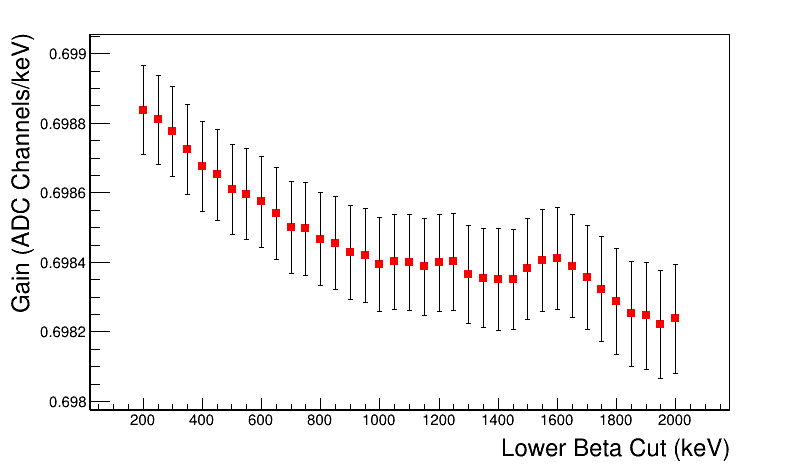
\includegraphics[width=0.7\textwidth]{MCLBCvbwmOffsetis10Applied20_gain.png}}
	\caption{The effect of the lower beta cut in a simulation when the applied offset is 10 units higher than the real offset.}
	\label{fig:MCoffset10applied20}
\end{figure}

This effect can be exploited to determine an offset using only the data. 
The size of the slope induced is linear compared to the offset. %Add figure here
By adjusting the offset and noting the slope of the $G_{SM}$ vs the lower beta cut and plotting against the offset, the location of zero slope can be calculated.
This graph is shown in figure \ref{fig:slopevoffset}.
\begin{figure}[!htb]
	\centerline{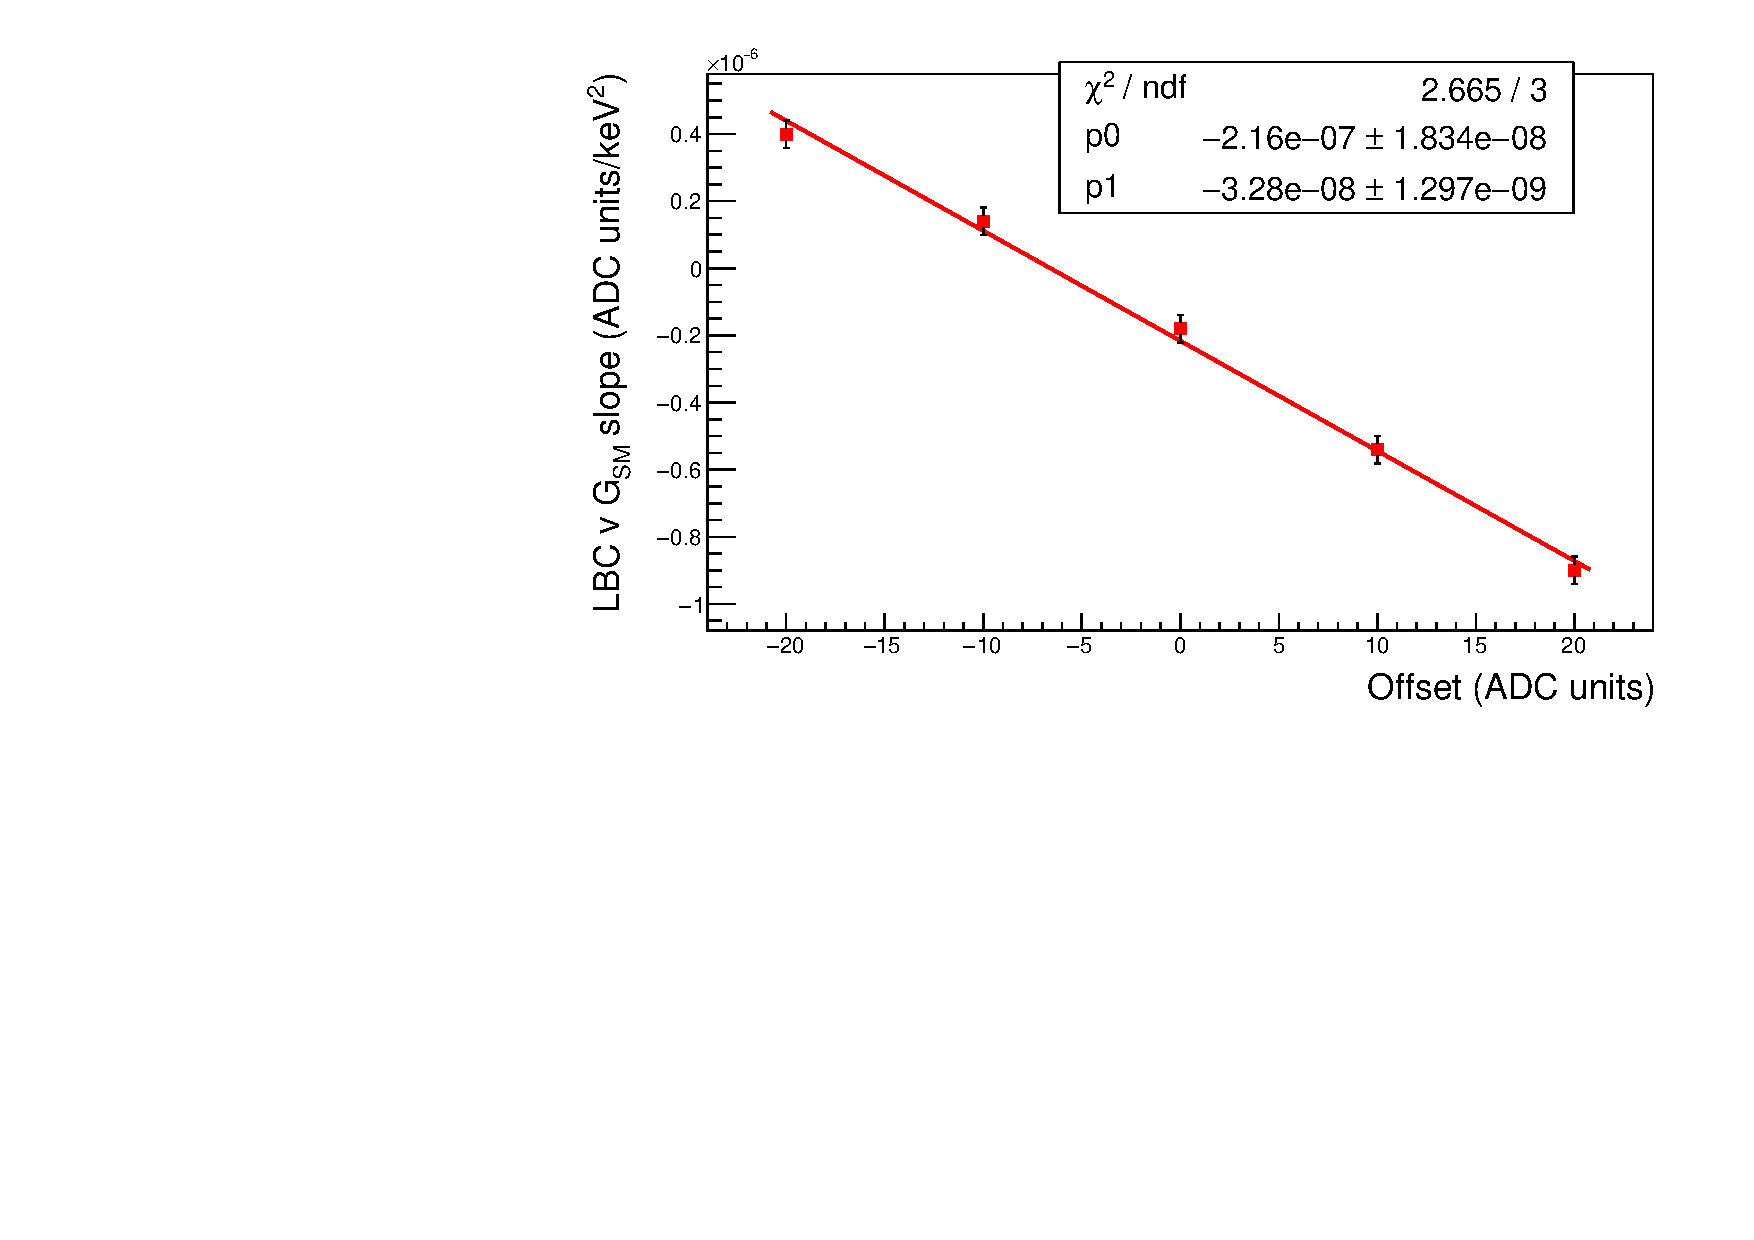
\includegraphics[width=0.70\textwidth]{fig_offsetvslopecurve_gain.pdf}}
	\caption{How the slope of the $G_{SM}$ vs LBC curve changes with offset.
		 A slope of 0 corresponds to an offset of -6.6}
	\label{fig:slopevoffset}
\end{figure}
The resulting $b_{WM}$ and $b_{GT}$ curves are seen in figure \ref{fig:offset0LBCeffect}.

\begin{figure}
    \centering
    \begin{minipage}{0.50\textwidth}
        \centerline{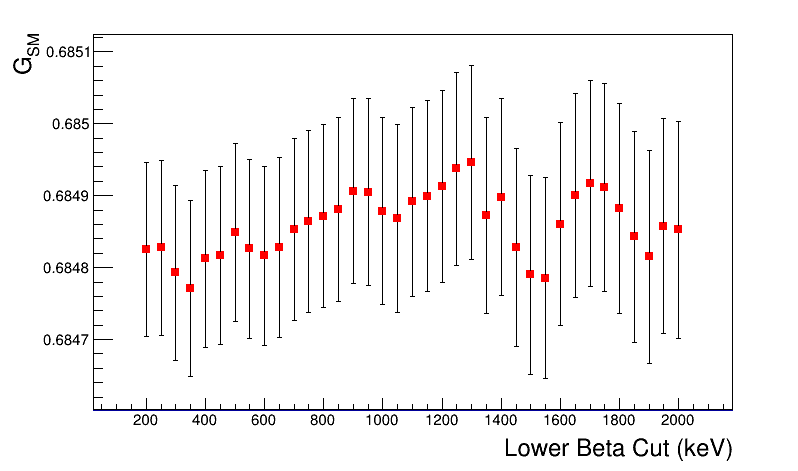
\includegraphics[width=0.9\textwidth]{CsILBCvGainSMOffsetism6p64histfit.png}}
    \end{minipage}\hfill
    \begin{minipage}{0.50\textwidth}
        \centerline{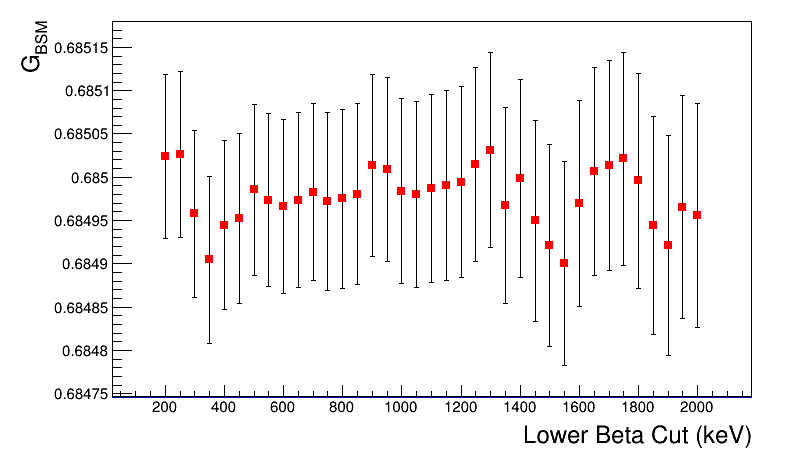
\includegraphics[width=0.9\textwidth]{CsILBCvGainBSMOffsetism6p64histfit.png}}
    \end{minipage}
    \caption{The depedence of the parameters to the start of the fit.
	     The offset here is -6.6.
    	     Both gains are indepedent of the start of the fit.}
    \label{fig:offset0LBCeffect}
\end{figure}

To estimate the uncertainty on the offset, the statistical uncertainty of the slope of the lines fit to the $b_{GT}$  was taken.
The offset was varied and how the slope of the line changed as the offset changed was recorded.
Then, the uncertainty of the slope was changed into an uncertainty on the offset using this information.
This gave an uncertainty of 0.1 on the offset.

The gain used in the fit is an average over the full run.
This gain shifts as 
Other effects are important. 


\subsubsection{The Convolution}

Another potential effect is if the detector resolution was applied incorrectly.
To test that, a Monte Carlo simulation was written.
The phase space in equation \ref{eq:phase_space} was multiplied by the shape factor in equation \ref{eq:shapefactor}.
This function was sampled $10^{9}$ times twice to build two histograms. 
Both histograms had a detector resolution applied as described in section \ref{sec:convolution}
One histogram was sampled a further $10^{6}$ times 10 times to build a sample data set.
The other convoluted histogram was used to fit the generated data set.
The first histogram's $A$ was fixed, while the second histogram's $A$ was adjusted.
When the sample data's $A$ matched the $A$ that were used, no dependence of $b_{WM}$ on the start of the fit was found.
When the $A$ of the data sample and the $A$, the first thing that happened was that the $b_{WM}$ changed.
If the $A$ differ by a factor of 2 or more, a shift in $b_{WM}$ appears.
However, this is much larger than any uncertainty in detector resolution.
The effect of a wrong detector resolution is negligible. 

\subsection{Upper Beta Cut Effect}

Changing where the fit ends has effectively no effect on the value either parameter.
An issue is that at small enough upper beta cut, there is nothing to fix the pile-up parameter on. 
This means that there could be correlations induced.
To avoid this, the  pre-fit was done, and the level of pile-up recorded.
The level of pile-up was fixed for the other fits across all upper beta cuts.
The lower beta cut was fixed to 250 keV in the fits. 
The effect is shown in figure \ref{fig:UBCEffect}.
Both parameters are flat after 5500 keV.

\begin{figure}
    \centering
    \begin{minipage}{0.50\textwidth}
        \centerline{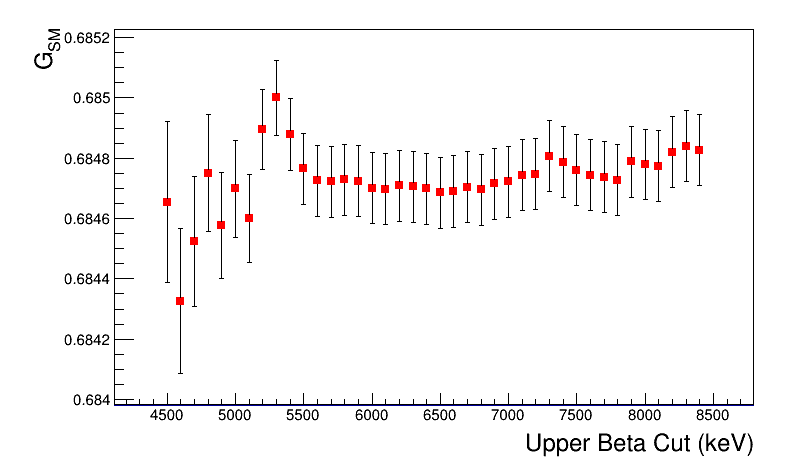
\includegraphics[width=0.9\textwidth]{CsIGSMvUBC4HistFit.png}}
    \end{minipage}\hfill
    \begin{minipage}{0.50\textwidth}
        \centerline{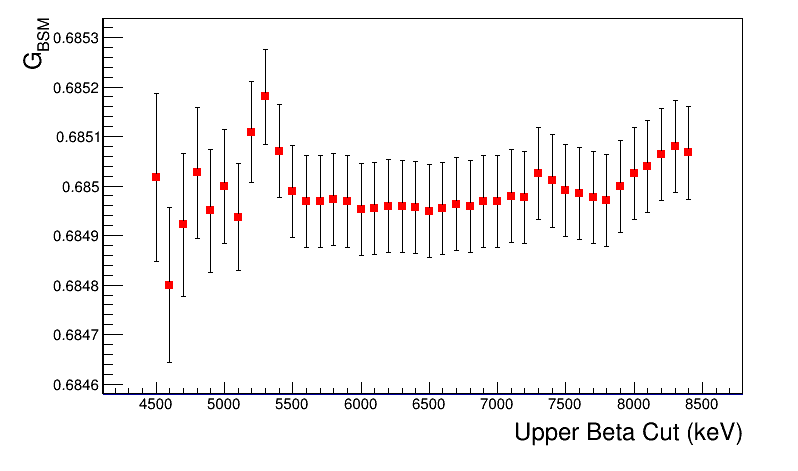
\includegraphics[width=0.9\textwidth]{CsIGBSMvUBC4HistFit.png}}
    \end{minipage}
    \caption{The effect of changing the upper beta cut.}
    \label{fig:UBCEffect}
\end{figure}

\subsection{Other Systematic Uncertainties}

The lower beta cut effect is the largest of the systematic uncertainties.
Many of the other systematic uncertainties are independent of the absolute value of $b_{GT}$.
To calculate these uncertainties, the lower beta cut was fixed to 250 keV.
The offset was set to -6.5, and the level of the beta-gamma sum spectrum was set to 1.
These parameters give the conditions in figure \ref{fig:offset0LBCeffect}.

For the calculation of the systematic uncertainties, one parameter at a time was adjusted.
The parameter was increased by one unit of the error on that parameter.
The fit was redone with the different parameter values.
The output $b_{WM}$ and $b_{GT}$ for the changes in the parameters were recorded.
The parameter then was then decreased by one unit of the error.
Half the difference of the output $b_{WM}$ and $b_{GT}$ were the systematic error.

As stated above, the different systematic uncertainties can be divided into three different categories. 
There are the systematic uncertainties due to the simulation inputs, which are summarized in table \ref{tab:simsyseffect}
These were all calculated by running the four histograms with $2 \times 10^{9}$ events each.

\begin{table}[!hbt]
	\centering
	\caption{Systematic uncertainties due to simulation inputs.}
		\begin{tabularx}{\textwidth}{RLLLL}
		Parameter Name & Parameter Value & Parameter Uncertainty & Systematic Uncertainty $b_{WM}$ & Systematic Uncertainty $b_{GT}$ \\ \hline
		Electron maximum total energy & 5900.864 $keV$ & 0.081 $keV$ & 0.2 & 0.0012\\
		Charge radius & 3.0055 $fm$ & 0.0021 $fm$  & 0.2 & 0.0003 \\
		\end{tabularx}
		\label{tab:simsyseffect}
\end{table}

The uncertainty due to the average mass $M_{ave}$ was ignored, as it is very small.
The value of the average mass used is $18621497.033 \pm 0.040$ keV.
Since this value appears in the denominator, and the uncertainty is so small, the effect of the uncertainty due to this average mass value is negligible. 
On the other hand, an uncertainty in the end point can have a larger effect.
The endpoint energy of the electron is only around 5 MeV.  

The systematic effects due to the fit inputs are shown in table \ref{tab:fitsyseffect}.
The systematic effect on the offset is linked to the lower beta cut effect and not listed yet.
The normalization of the beta-gamma sum spectrum is linked and not listed.
They still need to be investigated.
There is no systematic upper beta cut effect.

\begin{table}[!hbt]
	\centering
	\caption{Systematic uncertainties due to fit inputs.} 
		\begin{tabularx}{\textwidth}{RLLLL}
		Parameter Name & Parameter Value & Parameter Range or Uncertainty & Systematic Uncertainty on $b_{WM}$ & Systematic Uncertainty $b_{GT}$\\ \hline
 		Lower beta cut & 250 keV & 200 to 2000 keV & 5.5 & 0.0235 \\
		Offset & -6.5 & -6.6 to -6.4 & 0.3 & 0.0008 \\
		Binning of data histogram & 32 & 16 to 64 & 0.6 & 0.0003\\
		Binning of fitting histograms & 32 & 16 to 64 & 0.2 & 0.0007 \\ 
		Convolution & 1.112 & 0.008 &  0.3 & 0.0004 	 
		\end{tabularx}
		\label{tab:fitsyseffect}
\end{table}

Lastly, there are the systematic uncertainties due to the form factors inside the shape factor.
To calculate the systematic uncertainty on $b_{WM}$ due to $b_{GT}$, two fits one after another were done.
First, $b_{GT}$ was fit with the central value of $b_{WM}$
The resulting gain was recorded.
This gain was fixed, and the altered value of $b_{WM}$ applied and $b_{GT}$ was fit again.
The difference between the fitted values of $b_{GT}$ was recorded as a systematic uncertainty.
It was found that the systematic uncertainty of $b_{GT}$ depended on where the fit was started. 
This is another reason to start the fit as low as possible. 
These are summarized in table \ref{tab:formfactorsyseffect}

\begin{table}[!hbt]
	\centering
	\caption{Systematic uncertainties due to nuclear form factors.} 
		\begin{tabularx}{\textwidth}{RLLLLL}
		Parameter Name & Parameter Variable & Parameter Value & Parameter Uncertainty & Systematic Uncertainty $b_{WM}$ & Systematic Uncertainty $b_{GT}$ \\ \hline
		Weak magentism & $b_{WM}$ & 43.4 & 1.2 \cite{Min11} & N/A & 0.0034 \\
		Induced tensor form factor & $d$ & 40.5 &  3.7 \cite{Min11} & 0.2 & 0.0004 \\
		Fermi matrix element & $c_{1h}$ & 0.253 & 0.004 \cite{Min11} & 0.5  & 0.0017 \\
		Second forbidden matrix element & $c_{2h}$  & 0.755 $fm^{2}$ & 0.257 $fm^{2}$ \cite{Elm87} & 0.2 & 0.0011
		\end{tabularx}
		\label{tab:formfactorsyseffect}
\end{table}

The largest uncertainty is due to the lower beta cut effect.
The second largest uncertainty is due to the uncertainty of the weak magnetism.
\end{document}
